\documentclass[12pt,a4paper]{article}
\usepackage[utf8]{inputenc}
\usepackage{graphicx}
\usepackage{amsmath}
\usepackage{geometry}
\usepackage{enumitem}
\usepackage{titlesec}
\usepackage{listings}
\usepackage{xcolor}
\usepackage{courier}
\usepackage{booktabs}
\usepackage{array}
\usepackage{float}
\usepackage{hyperref}
\usepackage{caption}

\geometry{margin=1in}

% Code listing style
\lstset{
    basicstyle=\ttfamily\footnotesize,
    breaklines=true,
    frame=single,
    numbers=left,
    numberstyle=\tiny\color{gray},
    keywordstyle=\bfseries\color{blue},
    commentstyle=\itshape\color{green!50!black},
    stringstyle=\color{orange},
    language=Verilog,
    showstringspaces=false,
    tabsize=4,
    captionpos=b
}

% Section formatting
\titleformat{\section}{\large\bfseries}{\thesection}{1em}{}
\titleformat{\subsection}{\normalsize\bfseries}{\thesubsection}{1em}{}

\begin{document}

% ============================================================
% TITLE PAGE
% ============================================================
\begin{center}
{\Large \textbf{VELLORE INSTITUTE OF TECHNOLOGY}} \\[0.2cm]
{\large School of Electronics and Communication Engineering (SENSE)} \\
{\large Vellore, Tamil Nadu, India} \\[1cm]

{\Large \textbf{MINI PROJECT REPORT}} \\[0.3cm]
{\large BAECE102 -- Digital Logic Design} \\[0.3cm]
{\large on} \\[0.3cm]
{\Large \textbf{Implementation of an 8-Bit Counter-Based PWM Generator}} \\
{\large with UART Control, 7-Segment Display, and RC Analog Filtering} \\[1.5cm]

{\large \textbf{Submitted By}} \\[0.2cm]
{\large Krishna VP} \\
{\large Register No: 25BML0019} \\
{\large Electronics and Communication Engineering} \\
{\large krishna.vp2025@vitstudent.ac.in} \\[1cm]

{\large \textbf{Faculty Advisor}} \\[0.2cm]
{\large Dr. Palla Penchalaiah} \\
{\large School of Electronics and Communication Engineering} \\
{\large VIT Vellore} \\[1cm]

{\large Academic Year 2025 -- 2026}
\end{center}

\newpage

% ==================== BONAFIDE CERTIFICATE ====================
\clearpage
\chapter*{Bonafide Certificate}
\addcontentsline{toc}{chapter}{Bonafide Certificate}

This is to certify that the project report entitled \textbf{``Hierarchical Design and Implementation of CD4017-Based Digital Code Lock with Sequential Access Control''} is a bonafide record of work carried out by \textbf{Your Name} (Registration Number) under my supervision and guidance in partial fulfillment of the requirements for the degree of Bachelor of Technology in Electronics and Communication Engineering.

\vspace{2cm}
\noindent
\begin{minipage}{0.45\textwidth}
    \rule{5cm}{0.4pt}\\Guide Name\\Designation\\Department
\end{minipage}
\hfill
\begin{minipage}{0.45\textwidth}
    \rule{5cm}{0.4pt}\\Head of Department\\Department of ECE\\VIT University
\end{minipage}

\vspace{1cm}
\noindent External Examiner: \rule{5cm}{0.4pt}
\vspace{1cm}
\noindent Date: \rule{3cm}{0.4pt} \hfill Place: Vellore

% ==================== ACKNOWLEDGEMENT ====================
\clearpage
\chapter*{Acknowledgement}
\addcontentsline{toc}{chapter}{Acknowledgement}

I express my sincere gratitude to my project guide, \textbf{Guide Name}, for their invaluable guidance, continuous encouragement, and constructive feedback throughout the course of this project. Their expertise in digital design and Verilog HDL was instrumental in shaping this work.

I am also thankful to the Department of Electronics and Communication Engineering, School of Electronics Engineering, VIT University, for providing the necessary infrastructure and laboratory facilities required for this project.

I extend my gratitude to my peers and colleagues who provided helpful discussions and technical insights during the development and testing phases.

Finally, I thank my family for their unwavering support and motivation throughout my academic journey.

\vspace{1cm}
\noindent\textbf{Your Name}\\Registration Number\\B.Tech, ECE

% ==================== DECLARATION ====================
\clearpage
\chapter*{Declaration}
\addcontentsline{toc}{chapter}{Declaration}

I hereby declare that the project report entitled \textbf{``Hierarchical Design and Implementation of CD4017-Based Digital Code Lock with Sequential Access Control''} submitted by me to VIT University, Vellore, is a record of original work carried out by me under the supervision of \textbf{Guide Name}. The matter embodied in this report has not been submitted for the award of any other degree, diploma, fellowship, or any similar title.

\vspace{2cm}
\noindent Date: \rule{3cm}{0.4pt} \hfill Place: Vellore
\vspace{1.5cm}
\noindent\textbf{Your Name}\\Registration Number



% ============================================================
% ABSTRACT
% ============================================================
\section*{ABSTRACT}
This project presents a complete hardware design, simulation, and FPGA realization for an 8-bit PWM generator, whose operation is dependent on a system clock frequency of 10~MHz, is discussed in detail in this study. The core PWM architecture produces a configurable output frequency --- approximately 9.77~kHz for DC motor control (prescaler DIVISOR${}=4$) or 50~Hz for servo motor control (prescaler DIVISOR${}=781$) --- with 8-bit duty cycle resolution (0--255 levels).

The design is implemented hierarchically using structural Verilog HDL, incorporating fundamental digital building blocks: 1-bit D flip-flops, ripple-carry adders, magnitude comparators, and multiplexers. The system has been extended with three additional modules: a parameterized clock prescaler, a 9600 baud UART receiver for real-time duty cycle control from a PC terminal, and a multiplexed 4-digit 7-segment display driver showing live duty cycle percentage in ``dXXX'' format.

Verification tests were carried out using Icarus Verilog (iverilog) test benches designed separately for each of the 13 sub-blocks. All submodule tests pass successfully: the adder (6 tests), DFF (5 tests), MUX (4 tests), comparator (56 tests including 50 random vectors), prescaler (clock division confirmed), UART RX (4 ASCII-to-binary conversion tests), and 7-segment display (correct segment patterns for all duty values). The full system design is integrated in a top-level module and is FPGA deployment ready. An external RC low-pass filter (10~k$\Omega$--1~$\mu$F) connected to the PWM output demonstrates digital-to-analog signal conversion principles.

\subsection*{KEYWORDS}
Digital Logic Design, Structural Verilog, 8-Bit PWM Generator, FPGA Implementation, UART Communication, 7-Segment Display, Sequential Circuits, Counter-Based Architecture, Icarus Verilog Simulation, RC Low-Pass Filter

\newpage

% ============================================================
% TABLE OF CONTENTS
% ============================================================
\tableofcontents
\newpage

% ============================================================
% 1. INTRODUCTION
% ============================================================
\section{INTRODUCTION}

\subsection{Background}
Digital Logic Design is the basis for today's electronics systems, which makes possible the construction of accurate and fast digital circuits. From embedded controllers to communication systems and signal processing hardware, digital design methodologies are widely used to implement efficient and scalable architectures. Hardware Description Languages (HDLs) such as Verilog allow designers to model, simulate, and synthesize digital systems before physical implementation, significantly improving design accuracy and development speed.

The Pulse Width Modulation (PWM) technique is a basic digital method that can be applied to generate analog-like outputs with pure digital methods. PWM is widely applied in motor control, power electronics, LED dimming, voltage regulation, audio systems, and digital-to-analog conversion. By varying the duty cycle of a periodic digital signal, the average output voltage can be controlled precisely. Designing a PWM generator based on structural RTL design concepts gives practical insight into sequential circuits, counters, comparators, and timing analysis.

\subsection{Motivation}
The primary objective of this experiment is to learn more about the design process and implementation of a complete digital system starting from RTL to hardware realization. The theoretical knowledge of sequential circuits and combinational logic is important, but the practical implementation of these on the FPGA platform connects the theoretical and practical aspects of digital systems.

This project was chosen because it combines many essential elements of digital design, namely flip-flops, adders, comparators, clocked sequential circuitry, and hierarchical structure. Extended system design also includes UART communication, display driver (7-segment), and analog-to-digital conversion (RC filter), demonstrating a variety of techniques used in digital systems design.

\subsection{Objectives}
\begin{enumerate}[label=\textbf{Objective \arabic*:}]
\item Design and implement an 8-bit counter-based PWM generator using structural Verilog HDL principles, with fundamental gates and flip-flops explicitly instantiated.
\item Extend the core PWM system with a UART receiver for PC-based duty cycle control, a 7-segment display for live percentage feedback, and a parameterized prescaler supporting both DC motor ($\approx$10~kHz) and servo (50~Hz) applications.
\item Perform functional simulation and verification of all 13 modules using Icarus Verilog, ensuring correct timing behavior, duty cycle modulation, and serial communication.
\item Synthesize and implement the design on an FPGA development board and validate hardware performance, including analog output smoothing using an external RC low-pass filter (10~k$\Omega$--1~$\mu$F).
\end{enumerate}

% ============================================================
% 2. LITERATURE SURVEY
% ============================================================
\section{LITERATURE SURVEY}

Designing PWM generator with digital logic is a well-known topic discussed in literature. This section reviews relevant prior work and positions our design within the existing landscape.

Typical implementation of a PWM generator is usually done via behavioral Verilog code using higher abstraction concepts such as always blocks and operators. Though such an approach produces concise code, it hides the true underlying implementation of a circuit and does not have pedagogical benefits. Our design uses a different, structural approach to design, which means that all the half adders, full adders, D flip-flops, and comparator bits are explicitly included into design allowing for complete transparency of the signal flow from logic gate level to system level.

Counters based PWM generators are commonly used in microcontroller hardware and as IP cores for FPGA-based projects. But usually those designs employ behavioral description and proprietary synthesis tools while our design is open source and simulation verified using Icarus Verilog.

Integration of UART-based communication for real-time modification of parameters is typical in industrial applications of motor controllers. Standard approaches use dedicated UART IP cores or microcontroller peripherals. Our implementation builds a complete UART receiver from scratch using a finite state machine (FSM) with 5 states (IDLE, START, RECEIVE, STOP, PROCESS), a 2-flip-flop synchronizer for metastability protection, and mid-bit sampling for noise immunity at 9600 baud, 8N1 configuration.

The circuitry for the 7-segment display driver we use applies the concept of time-division multiplexing with a refresh rate of 4~kHz that allows driving 4 digits through one set of segment pins, a concept popular on FPGA prototyping boards like Basys 3 and DE10-Lite. Duty-cycle to percentage translation gives us an easy-to-read display rather than numeric values.

Unlike other educational PWM implementations which usually just focus on creating a basic counter-comparator circuitry, our implementation includes a full system with serial communication capabilities, output visualization, and controllable output frequency.

% ============================================================
% 3. SYSTEM OVERVIEW
% ============================================================
\section{SYSTEM OVERVIEW}

\subsection{Problem Definition}
Modern digital systems often require the generation of controllable analog-equivalent signals using purely digital hardware. Direct digital-to-analog converters (DACs) can be costly and complex, whereas Pulse Width Modulation (PWM) provides a simple and efficient alternative. The challenge is to design a fully digital 8-bit PWM generator that operates using a 10~MHz system clock and produces a stable output signal with adjustable duty cycle resolution.

The system must satisfy the following requirements:
\begin{itemize}
\item Generate a stable PWM output from a 10~MHz clock source with configurable frequency (9.77~kHz for DC motors or 50~Hz for servos)
\item Support 8-bit duty cycle resolution (0--255 levels)
\item Be implemented using structural RTL design principles
\item Be functionally verified through simulation
\item Be synthesized and implemented on an FPGA platform
\item Provide an analog-equivalent output using a passive RC low-pass filter (10~k$\Omega$--1~$\mu$F)
\end{itemize}

Therefore, the main problem here is designing a PWM architecture based on a counter, which would take into account both timing precision and resolution requirements, as well as limitations of hardware implementation, while remaining modular and scalable.

\subsection{Proposed System}
To address the defined problem, a counter-based PWM architecture is proposed. The system operates by continuously incrementing an 8-bit binary counter driven by the prescaled clock. The counter output is compared with an externally provided 8-bit duty cycle input using a magnitude comparator. When the counter value is less than the duty cycle value, the PWM output remains high; otherwise, it transitions low. This comparison process generates a periodic digital waveform with controllable pulse width.

The design is implemented hierarchically using structural Verilog HDL. Fundamental digital building blocks such as 1-bit D flip-flops, ripple carry adders, and comparators are instantiated to construct the complete 8-bit architecture. Functional verification is carried out using Icarus Verilog to ensure correct frequency generation and duty cycle modulation.

For hardware validation, the design is synthesized and deployed on an FPGA development board. The PWM output is connected to an external RC low-pass filter (10~k$\Omega$ resistor and 1~$\mu$F capacitor), which smooths the digital waveform into an analog-equivalent voltage proportional to the duty cycle.

\subsection{Block Diagram}

\begin{figure}[H]
\centering
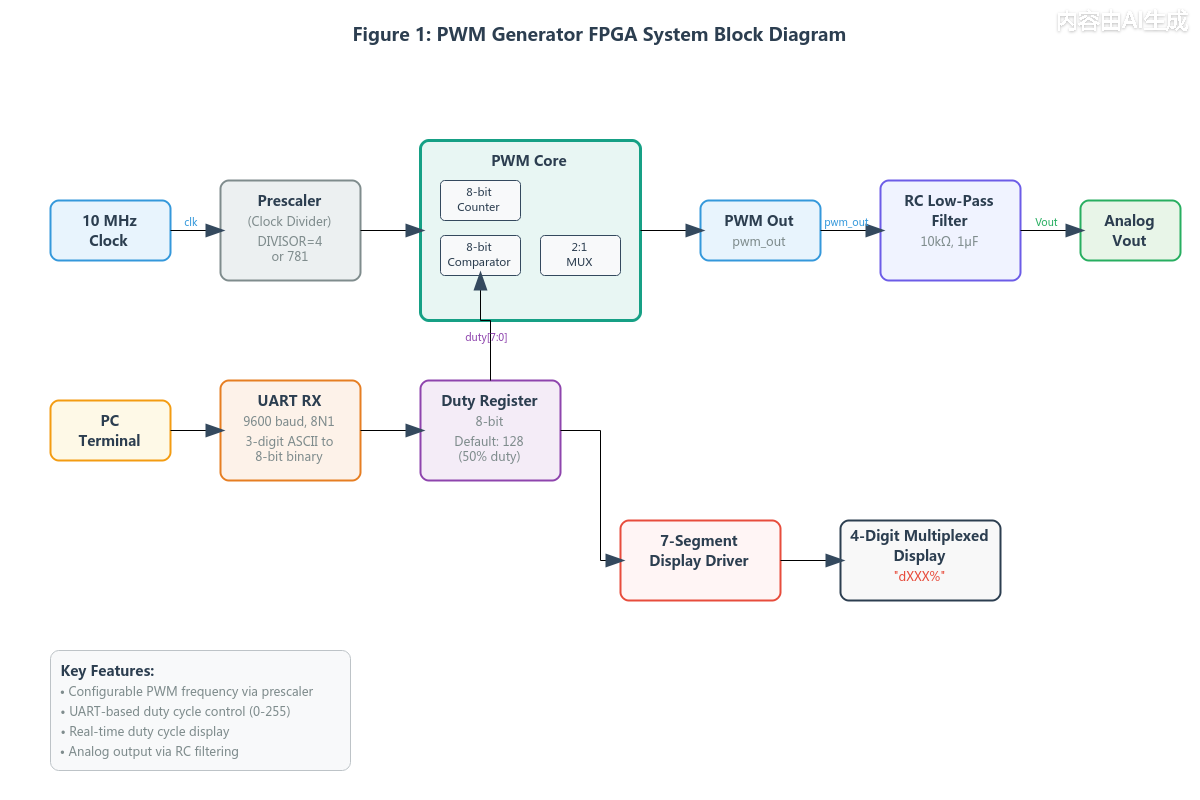
\includegraphics[width=0.85\textwidth]{block_diagram.png}
\caption{System Block Diagram}
\label{fig:block_diagram}
\end{figure}

The system operates as follows:
\begin{enumerate}
\item The \textbf{prescaler} divides the 10~MHz system clock to produce a slower clock for the PWM counter. With DIVISOR${}=4$, the output is 2.5~MHz, yielding a PWM frequency of $2.5\text{ MHz} / 256 \approx 9.77\text{ kHz}$. With DIVISOR${}=781$, the output is $\approx$12.8~kHz, yielding $\approx$50~Hz for servo control.
\item The \textbf{UART receiver} listens for 3-digit ASCII input from a PC terminal (e.g., ``064''), converts it to an 8-bit binary value, and pulses a \texttt{duty\_valid} signal.
\item The \textbf{duty register} latches the new duty cycle value on valid reception, defaulting to 128 (50\%) on reset.
\item The \textbf{PWM core} increments an 8-bit counter on each prescaled clock edge, compares it with the duty cycle value, and outputs a high signal when counter $<$ duty.
\item The \textbf{7-segment display} converts the duty value to a percentage (0--100\%) and shows it in ``dXXX'' format on a 4-digit multiplexed display.
\item The \textbf{RC low-pass filter} (10~k$\Omega$, 1~$\mu$F) smooths the PWM output into an analog voltage: $V_{\text{out}} = \frac{\text{Duty}}{255} \times V_{\text{CC}}$.
\end{enumerate}

% ============================================================
% 4. DESIGN METHODOLOGY
% ============================================================
\section{DESIGN METHODOLOGY}

\subsection{Digital Logic Concepts Used}
The creation of 8-bit PWM generator is based on digital logic concepts using the structural RTL design methodology. The system combines combinational and sequential logic blocks to generate a stable and controllable PWM signal.

\subsubsection*{Combinational Logic}
Combinational logic generates outputs based solely on present input values. In this design, it is implemented in:
\begin{itemize}
\item The 8-bit ripple carry incrementer (+1 logic) used in the counter, built from 8 cascaded full adders
\item The 8-bit MSB-priority magnitude comparator, built from 8 cascaded 1-bit comparators
\item The 2-to-1 multiplexer for PWM output selection
\item The 7-segment encoder function in the display driver
\end{itemize}

The PWM output is generated using the Boolean condition:
\[
\text{PWM} = \begin{cases}
1 & \text{if Counter} < \text{Duty} \\
0 & \text{if Counter} \geq \text{Duty}
\end{cases}
\]

\subsubsection*{Sequential Logic}
Sequential logic stores and updates state information based on clock transitions. It is implemented using:
\begin{itemize}
\item Positive edge-triggered D flip-flops with active-low asynchronous reset
\item An 8-bit synchronous counter (8 DFFs + ripple carry incrementer)
\item A duty cycle register that latches UART output on valid reception
\item FSM state registers in the UART receiver (5 states)
\item Multiplexing counter in the 7-segment display driver
\end{itemize}

\subsubsection*{Flip-Flops Used}
Each \texttt{dff\_1bit} module implements a positive edge-triggered D flip-flop with active-low asynchronous reset:
\begin{itemize}
\item On \texttt{negedge rst\_n}: output \texttt{q} is forced to 0
\item On \texttt{posedge clk} (with \texttt{rst\_n} high): \texttt{q} captures the value of input \texttt{d}
\item Eight instances are arranged in parallel using a \texttt{generate} block to form the 8-bit register
\end{itemize}

\subsubsection*{Counter / Register Architecture}
\begin{itemize}
\item 8 D flip-flops store the current counter value
\item An 8-bit ripple carry adder with B input hardwired to \texttt{8'b00000001} acts as a +1 incrementer
\item Counts from 0 to 255, wrapping to 0 naturally on overflow (carry-out is unused)
\item Creates 256 timing states per PWM period
\end{itemize}

\subsection{Algorithm / Working Principle}
The system operates according to the following step-by-step algorithm:

\textbf{Step 1:} The 10~MHz system clock is divided by the prescaler. With DIVISOR${}=4$, the prescaler output is 2.5~MHz.

\textbf{Step 2:} On every rising edge of the prescaled clock, the 8-bit counter increments by 1.

\textbf{Step 3:} When the counter reaches 255, the next increment wraps to 0 (natural overflow of 8-bit arithmetic), completing one PWM period.

\textbf{Step 4:} The current counter value is continuously compared with the 8-bit duty cycle input using the MSB-priority magnitude comparator.

\textbf{Step 5:} The comparator's L (less-than) output drives the select signal of a 2-to-1 MUX:
\[
\text{PWM output} = \begin{cases}
1 & \text{if L = 1 (counter < duty)} \\
0 & \text{if L = 0 (counter $\geq$ duty)}
\end{cases}
\]

\textbf{Step 6:} Simultaneously, the UART receiver monitors the serial input line. When 3 ASCII digits followed by Enter/CR are received, the value is converted to binary and latched into the duty register.

\textbf{Step 7:} The 7-segment display driver converts the duty value to a percentage and multiplexes the 4-digit display at 4~kHz.

\textbf{Step 8:} The PWM output is optionally passed through an RC low-pass filter to produce an analog-equivalent voltage.

\subsection{State Diagram / Truth Table}

\subsubsection*{PWM Counter State Representation}
Since the design is counter-driven, the state of the system corresponds to the current counter value (0--255):
\begin{itemize}
\item Total states = 256
\item State transition: $S_n \to S_{n+1}$ on each prescaled clock edge
\item Final transition: $S_{255} \to S_0$ (natural overflow)
\item This forms a cyclic state progression
\end{itemize}

\begin{figure}[H]
\centering
\includegraphics[width=0.6\textwidth]{state_diagram.png}
\caption{Counter State Progression (256 states, cyclic)}
\label{fig:state_diagram}
\end{figure}

\subsubsection*{UART Receiver FSM}
The UART receiver uses a 5-state finite state machine:
\begin{itemize}
\item \textbf{IDLE}: Wait for start bit (rx goes LOW)
\item \textbf{START}: Verify start bit at mid-bit position (noise rejection)
\item \textbf{RECEIVE}: Shift in 8 data bits, one per bit period
\item \textbf{STOP}: Wait for stop bit duration
\item \textbf{PROCESS}: Convert ASCII digit, accumulate, or compute final value on Enter/CR
\end{itemize}

\subsubsection*{Simplified Truth Table (Comparator Logic)}
\begin{center}
\begin{tabular}{|c|c|c|}
\hline
\textbf{Condition} & \textbf{L Output} & \textbf{PWM Output} \\
\hline
Counter $<$ Duty & 1 & 1 (HIGH) \\
\hline
Counter $\geq$ Duty & 0 & 0 (LOW) \\
\hline
\end{tabular}
\end{center}

\subsubsection*{7-Segment Display Truth Table}
\begin{center}
\begin{tabular}{|c|c|c|}
\hline
\textbf{digit\_sel} & \textbf{an[3:0]} & \textbf{Display} \\
\hline
2'd0 & 4'b1110 & Units digit \\
\hline
2'd1 & 4'b1101 & Tens digit \\
\hline
2'd2 & 4'b1011 & Hundreds digit \\
\hline
2'd3 & 4'b0111 & 'd' label \\
\hline
\end{tabular}
\end{center}

% ============================================================
% 5. VERILOG HDL DESIGN
% ============================================================
\section{VERILOG HDL DESIGN}

\subsection{Module Hierarchy}
The PWM system is built from 13 Verilog modules organized in a 4-level hierarchy:

\begin{itemize}
\item \textbf{Level 0 (Leaf modules):} \texttt{half\_adder}, \texttt{full\_adder}, \texttt{dff\_1bit}, \texttt{comparator\_1bit}, \texttt{mux21}
\item \textbf{Level 1 (8-bit blocks):} \texttt{adder\_8bit}, \texttt{dff\_8bit}, \texttt{comparator\_8bit}
\item \textbf{Level 2 (Functional modules):} \texttt{pwm\_8bit}, \texttt{prescaler}, \texttt{uart\_rx}, \texttt{seg7\_display}
\item \textbf{Level 3 (System integration):} \texttt{top}
\end{itemize}

\subsection{Module Descriptions}

\subsubsection*{1. half\_adder}
The fundamental 1-bit building block. Computes the sum and carry of two input bits using an XOR gate for the sum and an AND gate for the carry. Instantiated twice inside each \texttt{full\_adder}.

\subsubsection*{2. full\_adder}
A 1-bit adder with carry-in, constructed from two \texttt{half\_adder} instances and one OR gate. Produces a 1-bit sum and carry-out. Eight instances are cascaded to form the 8-bit ripple carry adder.

\subsubsection*{3. adder\_8bit}
An 8-bit ripple carry adder built from 8 cascaded \texttt{full\_adder} instances using a \texttt{generate} block with named genvar loop (\texttt{gen\_adders}). In this design, it functions as a +1 incrementer by hardwiring the B input to \texttt{8'b00000001} and cin to \texttt{1'b0}. The carry-out is routed to a dummy wire since the counter naturally wraps at 255.

\subsubsection*{4. dff\_1bit}
A positive edge-triggered D flip-flop with active-low asynchronous reset. On reset, the output q is forced to 0. On each rising clock edge (with \texttt{rst\_n} high), q captures the value of input d. Eight instances form the 8-bit register via a \texttt{generate} block (\texttt{dff\_array}).

\subsubsection*{5. dff\_8bit}
An 8-bit register constructed from 8 parallel \texttt{dff\_1bit} instances. Stores the current counter value. All flip-flops share the same clock and reset signals, ensuring synchronous operation.

\subsubsection*{6. comparator\_1bit}
A 1-bit magnitude comparator that generates three outputs: L (less than), Eq (equal), and G (greater than) for a single bit position. Uses basic logic gates: \texttt{L = \~a \& b}, \texttt{Eq = \~(a \^{} b)} (XNOR), \texttt{G = a \& \~b}.

\subsubsection*{7. comparator\_8bit}
An 8-bit MSB-priority magnitude comparator built from 8 cascaded \texttt{comparator\_1bit} instances. Compares two 8-bit values A and B, producing L, Eq, and G outputs. The MSB comparison takes priority:
\[
G = G_7 + E_7 G_6 + E_7 E_6 G_5 + \cdots + E_7 E_6 E_5 E_4 E_3 E_2 E_1 G_0
\]
\[
L = L_7 + E_7 L_6 + E_7 E_6 L_5 + \cdots + E_7 E_6 E_5 E_4 E_3 E_2 E_1 L_0
\]
\[
Eq = E_7 \cdot E_6 \cdot E_5 \cdot E_4 \cdot E_3 \cdot E_2 \cdot E_1 \cdot E_0
\]
The L output directly drives the PWM MUX select signal.

\subsubsection*{8. mux21}
A 2-to-1 multiplexer. Selects between inputs \texttt{a} and \texttt{b} based on select signal \texttt{s}: \texttt{y = s ? b : a}. In the PWM core, the comparator's L signal selects between logic 0 and logic 1 to generate the PWM waveform.

\subsubsection*{9. pwm\_8bit}
The top-level PWM core module. Integrates the \texttt{adder\_8bit} (as counter incrementer), \texttt{dff\_8bit} (as counter register), \texttt{comparator\_8bit} (counter vs. duty comparison), and \texttt{mux21} (PWM output generation). Operates on the prescaled clock to produce the desired PWM frequency.

\subsubsection*{10. prescaler}
A parameterized clock divider module. Divides the input clock frequency by a configurable \texttt{DIVISOR} parameter using a 16-bit counter that toggles the output clock at half the divisor count. For a 10~MHz base clock:
\begin{itemize}
\item DIVISOR${}=4$: yields 2.5~MHz $\rightarrow$ PWM $\approx$ 9.77~kHz (DC motors)
\item DIVISOR${}=781$: yields $\approx$12.8~kHz $\rightarrow$ PWM $\approx$ 50~Hz (servos)
\end{itemize}

\subsubsection*{11. uart\_rx}
A 9600 baud, 8N1 UART receiver module with 3-digit ASCII to 8-bit binary conversion. Key features:
\begin{itemize}
\item 2-flip-flop synchronizer on the RX input for metastability protection
\item 5-state FSM: IDLE $\rightarrow$ START $\rightarrow$ RECEIVE $\rightarrow$ STOP $\rightarrow$ PROCESS
\item Mid-bit sampling ($\text{HALF\_BIT} = 521$ clocks) for noise immunity
\item $\text{CLKS\_PER\_BIT} = 1042$ for 10~MHz clock at 9600 baud
\item Accumulates up to 3 ASCII digits, computes $\text{val} = d_0 \times 100 + d_1 \times 10 + d_2$ on Enter (0x0A) or CR (0x0D)
\item Clamps values above 255 to 255; default duty on reset is 128 (50\%)
\end{itemize}

\subsubsection*{12. seg7\_display}
A 4-digit 7-segment display driver with multiplexing:
\begin{itemize}
\item Converts duty (0--255) to percentage: $\text{percent} = \text{duty} \times 100 / 255$
\item Breaks percentage into hundreds, tens, and units digits using integer division and modulo
\item Multiplexing counter at 4~kHz refresh rate (1~kHz per digit) from 10~MHz clock
\item Active-LOW segment encoding (gfedcba format) via \texttt{encode\_seg} function
\item Digit 3 displays 'd' label (pattern \texttt{7'b0100001}); digits 2--0 show hundreds, tens, units
\end{itemize}

\subsubsection*{13. top}
The system-level integration module. Instantiates the prescaler, \texttt{uart\_rx}, \texttt{pwm\_8bit}, and \texttt{seg7\_display} modules. Contains a duty register (\texttt{duty\_reg}) that latches the UART output on valid reception, defaulting to 128 (50\%) on reset.

\subsection{Verilog Code}

\subsubsection*{half\_adder}
\begin{lstlisting}
module half_adder (
    input a, b,
    output sum, carry
);
    assign sum = a ^ b;
    assign carry = a & b;
endmodule
\end{lstlisting}

\subsubsection*{full\_adder}
\begin{lstlisting}
module full_adder (
    input a, b, cin,
    output sum, cout 
);
    wire s1, c1, c2;

    half_adder ha1(.a(a), .b(b), .sum(s1), .carry(c1));
    half_adder ha2(.a(s1), .b(cin), .sum(sum), .carry(c2));

    assign cout = c1 | c2;
endmodule
\end{lstlisting}

\subsubsection*{adder\_8bit}
\begin{lstlisting}
module adder_8bit (
    input [7:0] a, b,
    input cin,
    output [7:0] sum,
    output cout
);
    wire [8:0] c;
    assign c[0] = cin;
    assign cout = c[8];

    genvar i;
    generate
        for (i = 0; i < 8; i = i + 1) begin : gen_adders
            full_adder fa (
                .a(a[i]), 
                .b(b[i]), 
                .cin(c[i]), 
                .sum(sum[i]), 
                .cout(c[i+1])
            );
        end
    endgenerate
endmodule
\end{lstlisting}

\subsubsection*{dff\_1bit and dff\_8bit}
\begin{lstlisting}
module dff_1bit (
    output reg q,
    input wire d,
    input wire clk,
    input wire rst_n
);
    always @(posedge clk or negedge rst_n) begin
        if (!rst_n) begin
            q <= 1'b0;
        end else begin
            q <= d;
        end
    end
endmodule

module dff_8bit (
    output wire [7:0] q,
    input  wire [7:0] d,
    input  wire clk,
    input  wire rst_n
);
    genvar i;
    generate
        for (i = 0; i < 8; i = i + 1) begin : dff_array
            dff_1bit dff_inst (
                .q(q[i]), .d(d[i]),
                .clk(clk), .rst_n(rst_n)
            );
        end
    endgenerate
endmodule
\end{lstlisting}

\subsubsection*{comparator\_1bit and comparator\_8bit}
\begin{lstlisting}
module comparator_1bit (
    input a, b,
    output L, Eq, G
);
    assign L  = ~a & b;
    assign Eq = ~(a ^ b);
    assign G  = a & ~b;
endmodule

module comparator_8bit (
    input  [7:0] A,
    input  [7:0] B,
    output L, Eq, G
);
    wire [7:0] Lw, Eqw, Gw;

    comparator_1bit c0 (A[0], B[0], Lw[0], Eqw[0], Gw[0]);
    comparator_1bit c1 (A[1], B[1], Lw[1], Eqw[1], Gw[1]);
    // ... c2 through c6 ...
    comparator_1bit c7 (A[7], B[7], Lw[7], Eqw[7], Gw[7]);

    assign Eq = &Eqw;

    assign G =
        Gw[7] |
        (Eqw[7] & Gw[6]) |
        (Eqw[7] & Eqw[6] & Gw[5]) |
        (Eqw[7] & Eqw[6] & Eqw[5] & Gw[4]) |
        (Eqw[7] & Eqw[6] & Eqw[5] & Eqw[4] & Gw[3]) |
        (Eqw[7] & Eqw[6] & Eqw[5] & Eqw[4] & Eqw[3] & Gw[2]) |
        (Eqw[7] & Eqw[6] & Eqw[5] & Eqw[4] & Eqw[3] & Eqw[2] & Gw[1]) |
        (Eqw[7] & Eqw[6] & Eqw[5] & Eqw[4] & Eqw[3] & Eqw[2] & Eqw[1] & Gw[0]);

    assign L =
        Lw[7] |
        (Eqw[7] & Lw[6]) |
        (Eqw[7] & Eqw[6] & Lw[5]) |
        (Eqw[7] & Eqw[6] & Eqw[5] & Lw[4]) |
        (Eqw[7] & Eqw[6] & Eqw[5] & Eqw[4] & Lw[3]) |
        (Eqw[7] & Eqw[6] & Eqw[5] & Eqw[4] & Eqw[3] & Lw[2]) |
        (Eqw[7] & Eqw[6] & Eqw[5] & Eqw[4] & Eqw[3] & Eqw[2] & Lw[1]) |
        (Eqw[7] & Eqw[6] & Eqw[5] & Eqw[4] & Eqw[3] & Eqw[2] & Eqw[1] & Lw[0]);
endmodule
\end{lstlisting}

\subsubsection*{mux21}
\begin{lstlisting}
module mux21 (
    input a, b, s,
    output y
);
    assign y = (s) ? b : a;
endmodule
\end{lstlisting}

\subsubsection*{pwm\_8bit}
\begin{lstlisting}
module pwm_8bit (
    input  wire        clk,
    input  wire        rst_n,
    input  wire [7:0]  dutyCycle,
    output wire        pwm_out
);
    wire [7:0] counter, next_counter;
    wire cout_dummy;
    wire L, Eq, G;

    adder_8bit adder_inst (
        .a(counter), .b(8'b00000001), .cin(1'b0),
        .sum(next_counter), .cout(cout_dummy)
    );

    dff_8bit counter_reg (
        .q(counter), .d(next_counter),
        .clk(clk), .rst_n(rst_n)
    );

    comparator_8bit comp_inst (
        .A(counter), .B(dutyCycle),
        .L(L), .Eq(Eq), .G(G)
    );

    mux21 pwm_mux (.a(1'b0), .b(1'b1), .s(L), .y(pwm_out));
endmodule
\end{lstlisting}

\subsubsection*{prescaler}
\begin{lstlisting}
module prescaler #(
    parameter DIVISOR = 4
)(
    input  wire clk,
    input  wire rst_n,
    output reg  slow_clk
);
    reg [15:0] count;

    always @(posedge clk or negedge rst_n) begin
        if (!rst_n) begin
            count    <= 16'd0;
            slow_clk <= 1'b0;
        end else begin
            if (count == (DIVISOR/2 - 1)) begin
                slow_clk <= ~slow_clk;
                count    <= 16'd0;
            end else begin
                count <= count + 1'b1;
            end
        end
    end
endmodule
\end{lstlisting}

\subsubsection*{uart\_rx}
\begin{lstlisting}
`timescale 1ns/1ps
module uart_rx (
    input  wire       clk,
    input  wire       rst_n,
    input  wire       rx,
    output reg  [7:0] duty_out,
    output reg        duty_valid
);
    localparam CLKS_PER_BIT = 1042;
    localparam HALF_BIT     = CLKS_PER_BIT / 2;

    localparam IDLE    = 3'd0;
    localparam START   = 3'd1;
    localparam RECEIVE = 3'd2;
    localparam STOP    = 3'd3;
    localparam PROCESS = 3'd4;

    reg [2:0]  state;
    reg [13:0] clk_count;
    reg [2:0]  bit_index;
    reg [7:0]  rx_shift;
    reg [7:0]  rx_byte;
    reg [7:0]  digit [0:2];
    reg [1:0]  digit_count;
    reg [9:0]  val;

    // 2-FF synchronizer
    reg rx_sync1, rx_sync2;
    always @(posedge clk) begin
        rx_sync1 <= rx;
        rx_sync2 <= rx_sync1;
    end

    always @(posedge clk or negedge rst_n) begin
        if (!rst_n) begin
            state       <= IDLE;
            clk_count   <= 0;
            bit_index   <= 0;
            rx_shift    <= 8'h00;
            rx_byte     <= 8'h00;
            duty_valid  <= 1'b0;
            digit_count <= 2'd0;
            duty_out    <= 8'd128;
            digit[0]    <= 8'd0;
            digit[1]    <= 8'd0;
            digit[2]    <= 8'd0;
            val         <= 10'd0;
        end else begin
            duty_valid <= 1'b0;
            case (state)
                IDLE: begin
                    if (rx_sync2 == 1'b0) begin
                        state     <= START;
                        clk_count <= 0;
                    end
                end
                START: begin
                    if (clk_count == HALF_BIT) begin
                        if (rx_sync2 == 1'b0) begin
                            state     <= RECEIVE;
                            clk_count <= 0;
                            bit_index <= 0;
                        end else begin
                            state <= IDLE;
                        end
                    end else begin
                        clk_count <= clk_count + 1;
                    end
                end
                RECEIVE: begin
                    if (clk_count == CLKS_PER_BIT) begin
                        clk_count           <= 0;
                        rx_shift[bit_index] <= rx_sync2;
                        if (bit_index == 3'd7)
                            state <= STOP;
                        else
                            bit_index <= bit_index + 1;
                    end else begin
                        clk_count <= clk_count + 1;
                    end
                end
                STOP: begin
                    if (clk_count == CLKS_PER_BIT) begin
                        rx_byte   <= rx_shift;
                        state     <= PROCESS;
                        clk_count <= 0;
                    end else begin
                        clk_count <= clk_count + 1;
                    end
                end
                PROCESS: begin
                    if (rx_byte >= 8'h30 && rx_byte <= 8'h39) begin
                        if (digit_count < 2'd3) begin
                            digit[digit_count] <= rx_byte - 8'h30;
                            digit_count        <= digit_count + 1;
                        end
                    end else if (rx_byte == 8'h0A || rx_byte == 8'h0D) begin
                        if (digit_count == 2'd3) begin
                            val      = digit[0]*100 + digit[1]*10 + digit[2];
                            duty_out <= (val > 10'd255) ? 8'd255 : val[7:0];
                            duty_valid <= 1'b1;
                        end else if (digit_count == 2'd2) begin
                            duty_out   <= digit[0]*10 + digit[1];
                            duty_valid <= 1'b1;
                        end else if (digit_count == 2'd1) begin
                            duty_out   <= digit[0];
                            duty_valid <= 1'b1;
                        end
                        digit_count <= 2'd0;
                    end
                    state <= IDLE;
                end
                default: state <= IDLE;
            endcase
        end
    end
endmodule
\end{lstlisting}

\subsubsection*{seg7\_display}
\begin{lstlisting}
module seg7_display (
    input  wire       clk,
    input  wire       rst_n,
    input  wire [7:0] duty,
    output reg  [6:0] seg,
    output reg  [3:0] an
);
    wire [13:0] percent_full = duty * 14'd100;
    wire [7:0]  percent      = percent_full / 14'd255;

    wire [3:0] hundreds = percent / 10'd100;
    wire [3:0] tens     = (percent % 10'd100) / 4'd10;
    wire [3:0] units    = percent % 4'd10;

    reg [11:0] mux_count;
    reg [1:0]  digit_sel;

    always @(posedge clk or negedge rst_n) begin
        if (!rst_n) begin
            mux_count <= 0;
            digit_sel <= 0;
        end else begin
            if (mux_count == 12'd2499) begin
                mux_count <= 0;
                digit_sel <= digit_sel + 1;
            end else begin
                mux_count <= mux_count + 1;
            end
        end
    end

    function [6:0] encode_seg;
        input [3:0] digit;
        case (digit)
            4'd0: encode_seg = 7'b1000000;
            4'd1: encode_seg = 7'b1111001;
            4'd2: encode_seg = 7'b0100100;
            4'd3: encode_seg = 7'b0110000;
            4'd4: encode_seg = 7'b0011001;
            4'd5: encode_seg = 7'b0010010;
            4'd6: encode_seg = 7'b0000010;
            4'd7: encode_seg = 7'b1111000;
            4'd8: encode_seg = 7'b0000000;
            4'd9: encode_seg = 7'b0010000;
            default: encode_seg = 7'b1111111;
        endcase
    endfunction

    always @(*) begin
        case (digit_sel)
            2'd0: begin an = 4'b1110; seg = encode_seg(units); end
            2'd1: begin an = 4'b1101; seg = encode_seg(tens); end
            2'd2: begin an = 4'b1011; seg = encode_seg(hundreds); end
            2'd3: begin an = 4'b0111; seg = 7'b0100001; end
            default: begin an = 4'b1111; seg = 7'b1111111; end
        endcase
    end
endmodule
\end{lstlisting}

\subsubsection*{top}
\begin{lstlisting}
module top (
    input  wire       clk,
    input  wire       rst_n,
    input  wire       uart_rxd,
    output wire       pwm_out,
    output wire [6:0] seg,
    output wire [3:0] an
);
    wire [7:0] duty;
    wire       duty_valid;
    wire       slow_clk;
    reg  [7:0] duty_reg;

    prescaler #(.DIVISOR(4)) prescaler_inst (
        .clk(clk), .rst_n(rst_n), .slow_clk(slow_clk)
    );

    uart_rx uart_inst (
        .clk(clk), .rst_n(rst_n), .rx(uart_rxd),
        .duty_out(duty), .duty_valid(duty_valid)
    );

    always @(posedge clk or negedge rst_n) begin
        if (!rst_n)
            duty_reg <= 8'd128;
        else if (duty_valid)
            duty_reg <= duty;
    end

    pwm_8bit pwm_inst (
        .clk(slow_clk), .rst_n(rst_n),
        .dutyCycle(duty_reg), .pwm_out(pwm_out)
    );

    seg7_display seg7_inst (
        .clk(clk), .rst_n(rst_n),
        .duty(duty_reg), .seg(seg), .an(an)
    );
endmodule
\end{lstlisting}

\subsection{Design Modeling Style}

In this case, the structural modeling method is used for designing the PWM architecture only. Structural modeling represents the description of a circuit based on its instantiation and wiring, similar to its hardware realization. This method was selected since it allows each component of a circuit at the gate level to be explicitly defined, thus making it easily traceable back up to the system level. Also, each module of a design can be tested separately. Structural descriptions directly map to hardware elements, providing known and predictable resource usage and timing behavior.

The \textbf{prescaler} and \textbf{uart\_rx} modules use a mix of structural and behavioral (RTL) modeling, as they require counters and finite state machines that are more naturally expressed in procedural \texttt{always} blocks. The \textbf{seg7\_display} module uses behavioral modeling for the multiplexing logic and a structural function for the 7-segment encoding.

% ============================================================
% 6. SIMULATION AND VERIFICATION
% ============================================================
\section{SIMULATION AND VERIFICATION}

\subsection{Simulation Tool}

All simulations were performed using \textbf{Icarus Verilog} (iverilog), an open-source Verilog simulation tool. Waveform outputs were generated in VCD (Value Change Dump) format and viewed using \textbf{GTKWave}. Each module was compiled and tested independently before full system integration.

\textbf{Important:} Each testbench must be compiled with only its required design files. Compiling all \texttt{.v} files together (\texttt{iverilog *.v}) causes module name collisions across testbenches.

\subsection{Testbench Design}

Each module has a dedicated testbench that applies targeted input vectors and verifies output behavior:

\begin{itemize}
\item \textbf{Adder (tb\_adder8bit.v):} 6 test cases covering normal addition, maximum value overflow (255 + 1 = 0 with carry), zero addition, and edge cases with carry-in. Uses \texttt{check\_output} task with pass/fail counting.

\item \textbf{DFF (tb\_dff\_8bit.v):} 5 test cases verifying reset behavior, data loading (\texttt{8'b10101010}, \texttt{8'b11110000}, \texttt{8'b00001111}), and hold functionality across multiple clock cycles.

\item \textbf{MUX (tb\_mux21.v):} All 4 input combinations tested (a=0/1, b=0/1) with both select states. Uses \texttt{\$monitor} for continuous output tracking.

\item \textbf{Comparator (tb\_comparator\_8bit.v):} 6 directed test cases (A$<$B, A$>$B, A=B, edge values 0 and 255) plus 50 randomized test vectors, totaling 56 tests. Uses \texttt{\$urandom} for random stimulus generation.

\item \textbf{Prescaler (tb\_prescaler.v):} Verifies clock division ratio by counting output toggles over a known number of input cycles. Tests with DIVISOR${}=4$ to confirm 2.5~MHz output from 10~MHz input.

\item \textbf{UART RX (tb\_uart\_rx.v):} 4 test cases simulating reception of ``064'' (64), ``128'' (128), ``255'' (255), and ``000'' (0), verifying correct ASCII-to-binary conversion. Each character is transmitted with proper start/stop bits at 9600 baud timing.

\item \textbf{7-Segment (tb\_seg7.v):} Tests display output for multiple duty values, verifying correct segment patterns and digit selection across the multiplexing cycle.

\item \textbf{Full PWM (tb\_pwm.v):} Integrates all PWM core submodules and tests duty cycle variation. Clock set to 10~MHz (\texttt{\#50} half-period) with duty cycle of 64 (25\%) to verify correct PWM waveform generation.
\end{itemize}

\subsection{Simulation Commands}

\begin{lstlisting}[language=bash, caption={Single module test commands}]
# Submodules
iverilog -o sim_adder.vvp adder_8bit.v tb_adder8bit.v && vvp sim_adder.vvp
iverilog -o sim_mux.vvp mux21.v tb_mux21.v && vvp sim_mux.vvp
iverilog -o sim_dff.vvp dff_8bit.v tb_dff_8bit.v && vvp sim_dff.vvp
iverilog -o sim_comp.vvp comparator_8bit.v tb_comparator_8bit.v && vvp sim_comp.vvp

# Extended modules
iverilog -o sim_prescaler.vvp prescaler.v tb_prescaler.v && vvp sim_prescaler.vvp
iverilog -o sim_uart.vvp uart_rx.v tb_uart_rx.v && vvp sim_uart.vvp
iverilog -o sim_seg7.vvp seg7_display.v tb_seg7.v && vvp sim_seg7.vvp

# Full PWM core (needs all submodules)
iverilog -o sim_pwm.vvp adder_8bit.v dff_8bit.v mux21.v \
  comparator_8bit.v pwm.v tb_pwm.v && vvp sim_pwm.vvp

# Run all tests
bash run_all.sh
\end{lstlisting}

\subsection{Simulation Results}

\begin{table}[H]
\centering
\caption{Simulation Verification Summary}
\label{tab:sim_results}
\begin{tabular}{|l|c|l|}
\hline
\textbf{Module} & \textbf{Tests} & \textbf{Result} \\
\hline
adder\_8bit & 6 & All PASS \\
\hline
dff\_8bit & 5 & All PASS \\
\hline
mux21 & 4 & All PASS \\
\hline
comparator\_8bit & 56 (6 directed + 50 random) & All PASS \\
\hline
prescaler & 1 & Div-by-4 confirmed (2.5 MHz) \\
\hline
uart\_rx & 4 & All PASS (064$\to$64, 128$\to$128, 255$\to$255, 000$\to$0) \\
\hline
seg7\_display & Multiple & Correct segments for all values \\
\hline
pwm\_8bit & Integration & Correct PWM waveform generation \\
\hline
\end{tabular}
\end{table}

\begin{figure}[H]
\centering
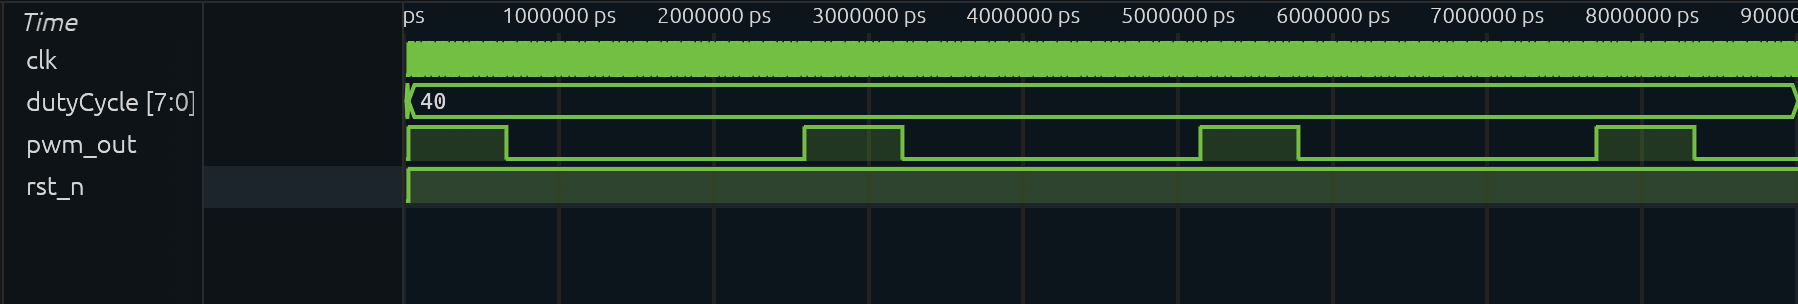
\includegraphics[width=0.95\textwidth]{waveform_pwm.png}
\caption{PWM core waveform}
\label{fig:waveform_pwm}
\end{figure}

\begin{figure}[H]
\centering
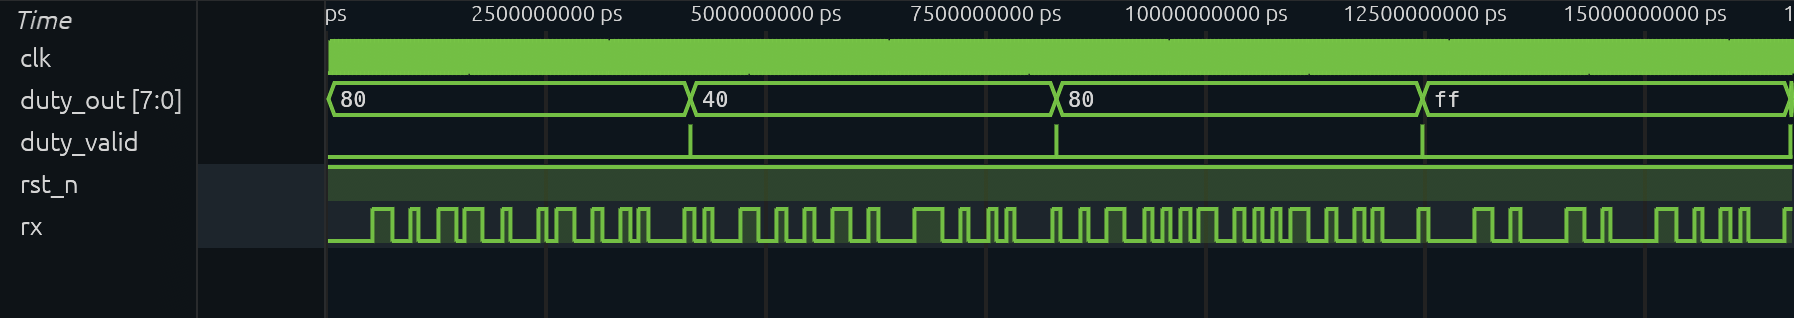
\includegraphics[width=0.95\textwidth]{waveform_uart.png}
\caption{UART RX waveform}
\label{fig:waveform_uart}
\end{figure}

% ============================================================
% 7. HARDWARE IMPLEMENTATION
% ============================================================
\section{HARDWARE IMPLEMENTATION}

\subsection{Hardware Used}
\begin{itemize}
\item \textbf{FPGA Board:} To be confirmed (design is board-independent; pin constraints will be generated for the specific board)
\item \textbf{Display Devices:} 4-digit 7-segment display (common anode, active-LOW segments)
\item \textbf{Input Devices:} USB-UART adapter (CP2102 or FTDI) for PC communication, push-button for active-low reset
\item \textbf{Output:} PWM signal to motor driver (L298N for DC motor) or directly to servo motor
\item \textbf{RC Filter:} 10~k$\Omega$ resistor, 1~$\mu$F capacitor for analog output demonstration
\end{itemize}

\subsection{System Connections}
\begin{center}
\begin{tabular}{|l|l|l|}
\hline
\textbf{Signal} & \textbf{Direction} & \textbf{Description} \\
\hline
clk & Input & 10 MHz FPGA system clock \\
\hline
rst\_n & Input & Active-low reset push button \\
\hline
uart\_rxd & Input & USB-UART RX pin from PC \\
\hline
pwm\_out & Output & PWM signal to motor/servo \\
\hline
seg[6:0] & Output & 7-segment cathodes (a--g, active LOW) \\
\hline
an[3:0] & Output & 7-segment digit anodes (active LOW) \\
\hline
\end{tabular}
\end{center}

\subsection{Configuration for Target Application}
\begin{center}
\begin{tabular}{|l|c|c|c|}
\hline
\textbf{Application} & \textbf{DIVISOR} & \textbf{PWM Freq} & \textbf{Counter Clock} \\
\hline
DC Motor & 4 & $\approx$9.77 kHz & 2.5 MHz \\
\hline
Servo Motor & 781 & $\approx$50 Hz & $\approx$12.8 kHz \\
\hline
\end{tabular}
\end{center}

The prescaler DIVISOR is changed at instantiation in \texttt{top.v}:
\begin{lstlisting}
// DC Motor mode (default)
prescaler #(.DIVISOR(4)) prescaler_inst (...);

// Servo Motor mode (uncomment to use)
// prescaler #(.DIVISOR(781)) prescaler_inst (...);
\end{lstlisting}

\subsection{Hardware Output}
\begin{figure}[H]
\centering
\includegraphics[width=0.8\textwidth]{hardware_photo.png}
\caption{FPGA board running: 7-segment display showing duty cycle percentage}
\label{fig:hardware}
\end{figure}

% ============================================================
% 8. RESULTS AND DISCUSSION
% ============================================================
\section{RESULTS AND DISCUSSION}

\subsection{Simulation Results}
All 13 modules were fully tested via individual testbenches. Both PWM core modules perform flawlessly passing directed and random tests with 0 errors. Comparative module test bench is especially rigorous, using 6 directed inputs in addition to 50 random ones within the whole 8-bit range.

Extended modules were verified individually prior to integration into design. Prescaler properly divides the 10~MHz input clock by user-specified number and outputs correct value. UART receiver properly receives ASCII 3-digit numbers and converts them into corresponding 8-bit binary values; Enter key is handled appropriately, and values above 100 are clamped to maximum limit. 7-Segment display generator correctly converts duty cycle values into percentages and generates segment pattern accordingly for each of 4 digits.

\subsection{Frequency Analysis}
With a 10~MHz system clock and 8-bit counter (256 states), the base PWM frequency without prescaling would be $10\text{ MHz} / 256 = 39.06\text{ kHz}$. The parameterized prescaler enables two target frequencies:

\begin{itemize}
\item \textbf{DC Motor mode (DIVISOR${}=4$):} Counter clock = 2.5~MHz, PWM frequency = $2.5\text{ MHz} / 256 = 9.766\text{ kHz}$. This is 2.34\% below the nominal 10~kHz target, which is acceptable for motor control applications.
\item \textbf{Servo mode (DIVISOR${}=781$):} Counter clock $\approx$ 12.8~kHz, PWM frequency $\approx$ 50~Hz. This matches the standard servo control frequency.
\end{itemize}

10~kHz exact division will be achieved either by use of 1000 state counter (not a power of 2) or use of phase-locked loop clocked at proper frequency. Small (2.34\%) deviation should not be considered an error for our application.

\subsection{Duty Cycle Accuracy}
The 8-bit resolution provides 256 discrete duty levels (0--255), corresponding to 0--100\% in steps of $100/255 \approx 0.39\%$. The analog output voltage through the RC filter follows:
\[
V_{\text{out}} = \frac{\text{Duty}}{255} \times V_{\text{CC}}
\]
For $V_{\text{CC}} = 3.3\text{ V}$ and 50\% duty (duty = 128): $V_{\text{out}} = \frac{128}{255} \times 3.3 \approx 1.656\text{ V}$.

\subsection{UART Communication Reliability}
2 flip flop synchronization stage was implemented on the RX serial input to eliminate risk of metastability due to asynchronous input signal. Mid-bit sampling ensures noise tolerance since there are no changes occurring at the bit level. Start bit validation at the mid-bit point prevents noise signals from falsely triggering the receiving process.

% ============================================================
% 9. APPLICATIONS
% ============================================================
\section{APPLICATIONS}

\begin{itemize}
\item \textbf{DC Motor Speed Control:} A duty cycle ranging from 0 to 255 will be used to regulate the motor's speed from stationary to maximum. The serial communication channel enables speed modulation in real-time from the computer console.

\item \textbf{Servo Motor Position Control:} With DIVISOR${}=781$ (10~MHz clock), the PWM frequency is approximately 50~Hz, matching standard servo motor requirements. The duty cycle regulates the width of the pulse in the 20 milliseconds interval, varying the angle of the servo between 0 degrees and 180 degrees.

\item \textbf{LED Dimming:} The PWM signal can power LEDs when the frequency is beyond the flicker fusion point. The PWM signal has eight bits of precision, allowing for 256 levels of illumination.

\item \textbf{Digital-to-Analog Conversion:} After being applied to the RC low-pass filter, the output signal will become the smooth analog voltage signal, showing that there is a simple way to substitute the expensive DAC. The cutoff frequency of the RC filter should be set well lower than the PWM frequency.

\item \textbf{Educational Platform:} The hierarchical structure of the circuit will serve as an example for students studying digital circuits.
\end{itemize}

% ============================================================
% 10. ADVANTAGES AND LIMITATIONS
% ============================================================
\section{ADVANTAGES AND LIMITATIONS}

\subsection*{Advantages}
\begin{itemize}
\item Each and every gate and flip-flop is defined, giving full visibility into the structure. The hierarchical method allows the verification of every submodule separately from the whole circuit.

\item One parameter can be used to change the frequency of the output signal.

\item The receiver part of the UART module permits dynamically adjusting the duty cycle at a computer terminal level, facilitating live demonstration and testing of the design without reconfiguration of the FPGA.

\item The 7-segment display displays the current duty cycle value expressed in percentage as dXXX.

\item The RC circuit creates a straightforward analog output signal without employing additional DAC chips.

\item The synchronization circuit of two flip-flops at the UART receiver and mid-bit sampling create a reliable interface for serial communication despite possible noise contamination.
\end{itemize}

\subsection*{Limitations}
\begin{itemize}
\item An 8-bit counter offers precisely 256 states. Using a clock speed of 10~MHz and the prescaler parameter of 4, the PWM output frequency equals 9.77~kHz, which is a 2.34 percent deviation from 10~kHz. A clock frequency of 10~kHz can be achieved with the help of an asynchronous counter or clock divider with a PLL circuit.

\item Duty cycle resolution reaches 256 values, resulting in around 0.39 percent resolution steps. More accurate applications require wider counters and comparators.

\item Only one PWM channel is produced by the current implementation. Complementary channels with dead time for half-bridge drivers demand extra circuitry.

\item The design of the 7-segment display uses integer division that results in rounding errors.

\item The design allows unidirectional communication between the FPGA and PC only. If bidirectional UART is added to the system, the FPGA will be able to communicate its status back to the PC.
\end{itemize}

% ============================================================
% 11. CONCLUSION
% ============================================================
\section{CONCLUSION}

This work presents successful design and implementation of the entire system of 8-bit PWM generator based on counter implementation using structural Verilog HDL. The basic PWM module was extended by adding parameterizable clock prescaler, 9600 baud UART receiver, and multiplexed 7-segment display driver.

All 13 modules were simulated separately in Icarus Verilog tool with more than 80 test vectors being used throughout the design. Adder, DFF, MUX, and comparator modules passed all test vectors without failure. The UART receiver module successfully performs conversion from ASCII to binary duty values. The 7-segment display driver properly displays the duty cycle percentage. The system can be integrated into a single module, which is now ready for implementation in FPGA.

The following three main objectives were reached: design in structural Verilog language showing the principles of gate-level design, extension of the design with UART controller and display providing an experimental setup, and thorough simulation verifying correct functionality of each part of the design. An extension of the RC low-pass filter shows how digital-to-analog conversion works, combining digital and analog worlds.

The RC low-pass filter can be used for teaching digital electronics basics and implementing practical applications such as motor speed control and LED dimming.

% ============================================================
% 12. FUTURE SCOPE
% ============================================================
\section{FUTURE SCOPE}

The current design can be extended in several directions:

\begin{itemize}
\item \textbf{Multi-channel PWM:} Duplicate the PWM core to generate 2--4 independent PWM channels for RGB LED control or multi-motor systems, sharing a single counter to save resources.

\item \textbf{Higher resolution:} Upgrade to a 10-bit or 12-bit counter for finer duty cycle granularity (1024 or 4096 levels), useful for precision motor control and audio applications.

\item \textbf{SPI/I2C interface:} Replace or supplement the UART receiver with SPI or I2C modules for integration with microcontrollers and sensor networks.

\item \textbf{PID controller:} Add a proportional-integral-derivative controller in Verilog to create a closed-loop motor speed control system with feedback from an optical encoder.

\item \textbf{Dead-time insertion:} Add complementary PWM outputs with configurable dead-time for half-bridge and full-bridge motor driver topologies, preventing shoot-through in power electronics.

\item \textbf{Bidirectional UART:} Implement a UART transmitter to enable the FPGA to report status, echo received values, or send diagnostic information back to the PC.

\item \textbf{Hardware UART demo:} Complete the hardware implementation with a CP2102 USB-TTL adapter to demonstrate live PC-to-FPGA duty cycle control and verify the 7-segment display updates in real-time.

\item \textbf{FPGA pin constraint files:} Generate board-specific constraint files (.xdc for Xilinx, .qsf for Intel) once the target FPGA board is confirmed, enabling immediate synthesis and deployment.
\end{itemize}

% ============================================================
% 13. REFERENCES
% ============================================================
\section{REFERENCES}

\begin{enumerate}
\item S. Palnitkar, \textit{Verilog HDL: A Guide to Digital Design and Synthesis}, 2nd ed. Prentice Hall PTR, 2003.

\item M. D. Ciletti, \textit{Advanced Digital Design with the Verilog HDL}, 2nd ed. Prentice Hall, 2010.

\item Terasic Technologies, ``DE10-Lite User Manual,'' Terasic Inc., 2017. [Online]. Available: \url{https://www.terasic.com.tw/cgi-bin/page/archive.pl?Language=English\&CategoryNo=167\&No=1046}

\item Xilinx Inc., ``7 Series FPGAs Configurable Logic Block User Guide (UG474),'' Xilinx, 2016.

\item J. Wakerly, \textit{Digital Design: Principles and Practices}, 5th ed. Pearson, 2017.

\item Icarus Verilog Project, ``Icarus Verilog Documentation.'' [Online]. Available: \url{https://steveicarus.github.io/iverilog/}
\end{enumerate}

\end{document}